%!TEX root = index.tex
\section{Cycle de développement logiciel}

Les cycles de développement des systèmes dans l'ingénierie des systèmes sont les processus de création ou de modification de systèmes d'information et les modèles et méthodes utilisés pour développer ces systèmes. En génie logiciel, ce concept sous-tend de nombreux types de méthodologies, et ces méthodes constituent le cadre pour la planification et le contrôle de la création d'un système d'information \cite{cycle}.

Les systèmes informatiques sont complexes et souvent (surtout avec la hausse récente de l'architecture orientée services) relient plusieurs systèmes traditionnels fournis par de différents fournisseurs de logiciels. Pour gérer ce niveau de complexité, un certain nombre de modèles ou de méthodes de gestion de cycle de vie logiciel ont été créés, tels que « cascade », « concourant », « spirale », « développement agile de logiciels », parmi d'autres.

\begin{figure}[H]
\begin{center}
    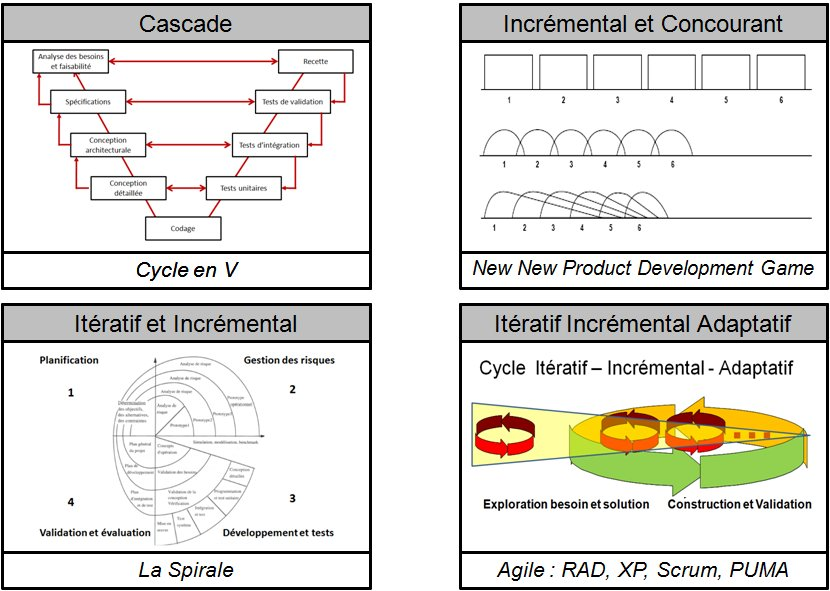
\includegraphics[scale=0.4]{img/cycles-basiques}
    \caption{Les principales cycles de développement logiciel}
	\label{cycles-basiques}
\end{center}
\end{figure}

\subsection{Les grandes familles de cycle de développement}

\subsubsection{Modèle en cascade}

Les phases traditionnelles de développement en cascade sont effectuées simplement les unes après les autres, avec un retour sur les précédentes. Le processus de développement utilisant un cycle en cascade exécute des phases qui produisent des livrables définis au préalable, se terminent à une date précise et seulement lorsque les livrables sont jugés satisfaisants lors d'une étape de validation-vérification.

\begin{figure}[H]
\begin{center}
    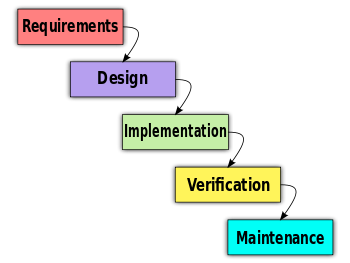
\includegraphics[scale=0.5]{img/waterfall}
    \caption{Le modèle en cascade}
	\label{waterfall}
\end{center}
\end{figure}

\subsubsection{Cycle en spirale}

Par l'implémentation de versions successives, le cycle recommence en proposant un produit de plus en plus complet et dur. En effet, le début de chaque itération comprend une phase d'analyse des risques. Ceci est rendu nécessaire par le fait que, lors d'un développement cyclique, il y a plus de risques de devoir défaire à une telle itération ce qu'on a fait à la précédente.

\begin{figure}[h]
\begin{center}
    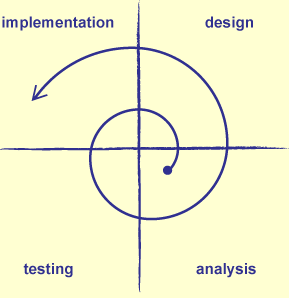
\includegraphics[scale=0.5]{img/spiral-model}
    \caption{Le cycle en spirale}
	\label{spiral-model}
\end{center}
\end{figure}

\subsubsection{Cycle itératif}

Toutes les méthodes Agiles, tels que ASD, FDD, Crystal, Scrum ou \textit{extreme programming},  débutent par des phases séquentielles, courtes mais bien réelles, d'exploration, d'architecture et de planning. Un usage totalement itératif de ces méthodes n'est cependant pas exclu mais ne peut s'appliquer qu'à de très petits projets. En fait, l'idée est de livrer au plus tôt quelque chose qui puisse être testé par le client. On peut en effet réaliser plusieurs itérations sur une documentation telle que l'architecture. 

\begin{figure}[h]
\begin{center}
    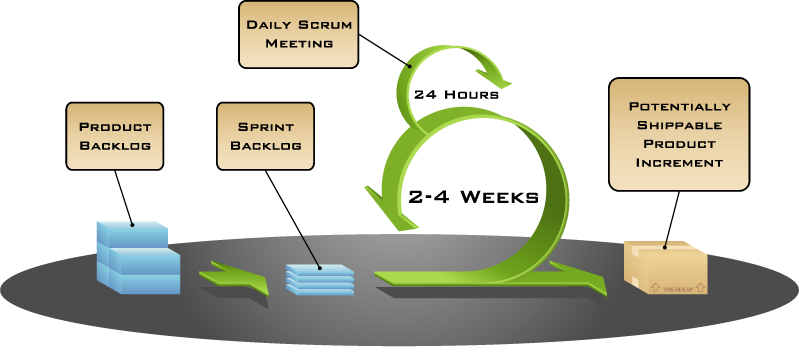
\includegraphics[scale=0.5]{img/scrum}
    \caption{Le processus itératif Agile de type Scrum}
	\label{scrum}
\end{center}
\end{figure}

\subsection{Le cycle de développement à Asert}\label{cycle}

L'entreprise d'accueil ne suit pas l'une des méthodes traditionnelles de processus de développement logiciel. En effet, les directives les plus importantes de toutes les méthodes sont prises en compte lors de la planification du projet, mais la structure globale varie selon le client, la taille et l'équipe.

En général, les étapes initiales des projets commencent très similaires au cycle cascade, avec la spécification des exigences du projet, entre le chef de projet et le client, avec l'aide de l'analyste de systèmes ; la conception des structures du projet, par l'architecte logiciel et l'analyste ; et le codage, par le développeur. Ensuite, le processus devient plus similaire aux méthodes agiles, avec l'intégration de versions préliminaires (alpha, beta, etc.) de la solution et avec des tests hebdomadaires. Finalement, une fois le projet est livré, les routines de maintenance se font périodiquement dans l'année. La documentation de projet n'est pas exhaustive, comme souvent les projets en cascade le demandent, mais un rapport final est livré au cliente avec le logiciel.

Du point de vue d'un projet en cours d'exécution, qui était déjà dans la phase de construction et codage, malheureusement je n'ai pas pu assister à toutes les étapes du cycle de vie du produit. Tout de même, le code du système a été revu plusieurs fois par le client lors de mon séjour à l'entreprise. De petites modifications ont dû être faites, mais cela n'a pas retardé énormément le développement.